% 导言区
\documentclass{ctexart}%ctexbook, ctexrep

%\usepackage{ctex}

% 导言区: \usepackage{graphicx}
% 语  法: \includegraphics[< 选项 >]{< 文件名 >}
% 格  式: EPS, PDF, PNG, JPG, BMP
\usepackage{graphicx}
\graphicspath{{figure/},}%图片在当前目录下的figure文件夹中

% 正文区(文稿区)
\begin{document}
	\LaTeX{}中的插图:
	
	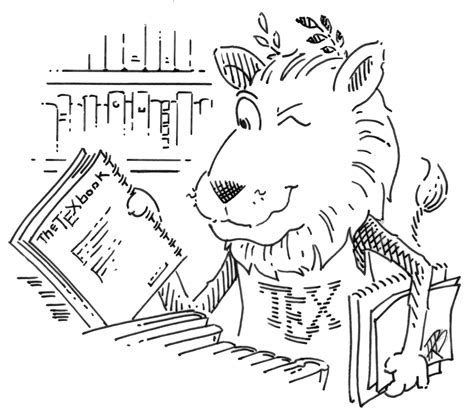
\includegraphics{lion}
	
\includegraphics{liang}
	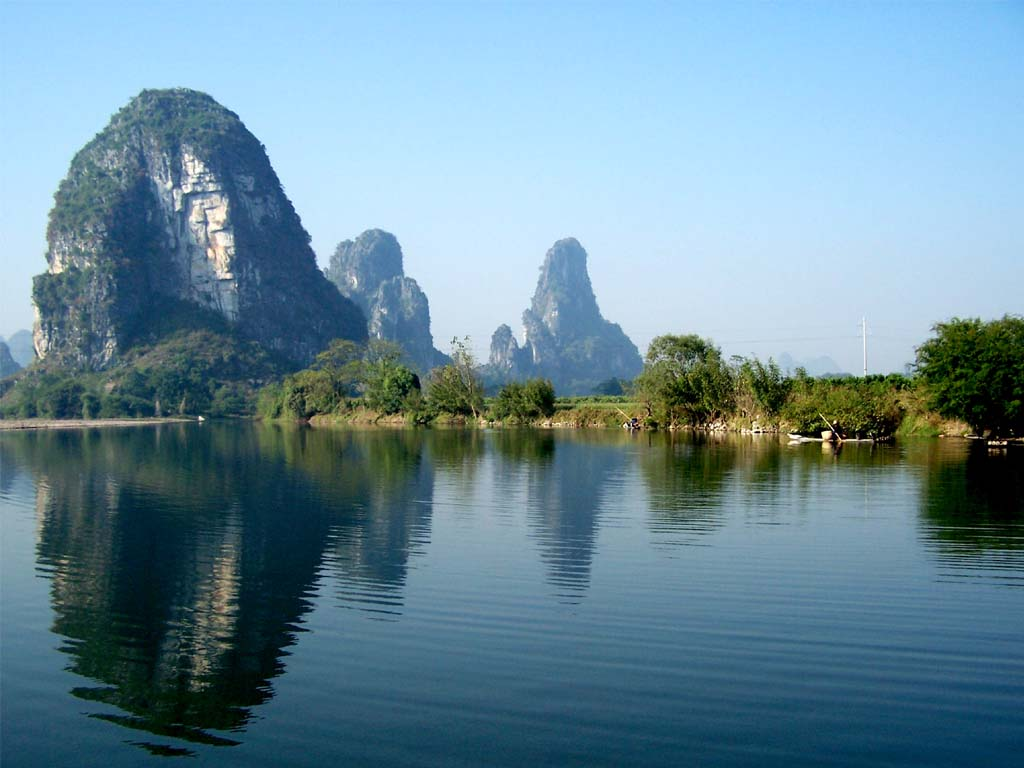
\includegraphics{guilin}
	
    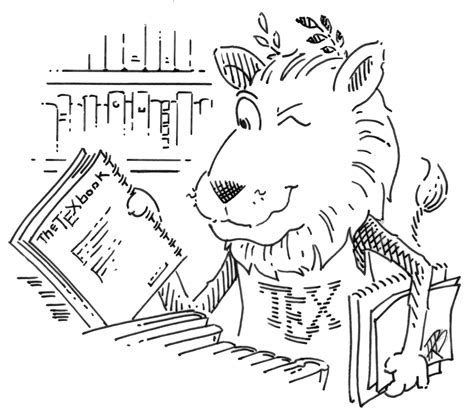
\includegraphics[scale=0.3]{lion}
	
\includegraphics[scale=0.3]{liang}
	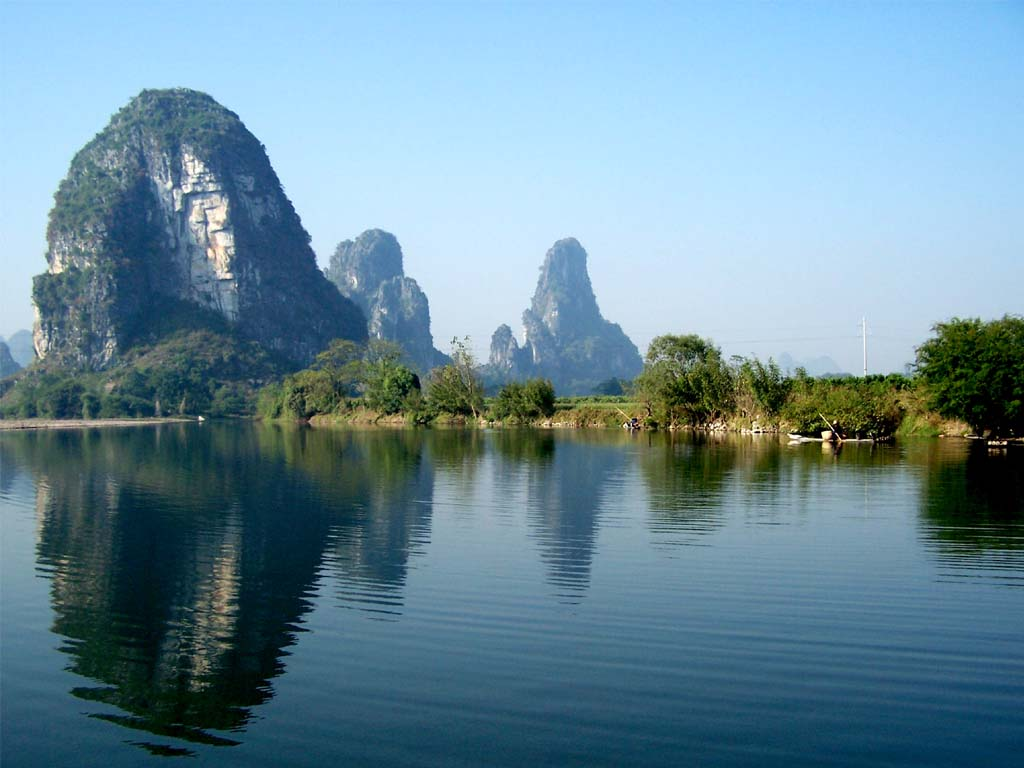
\includegraphics[scale=0.3]{guilin}
	
	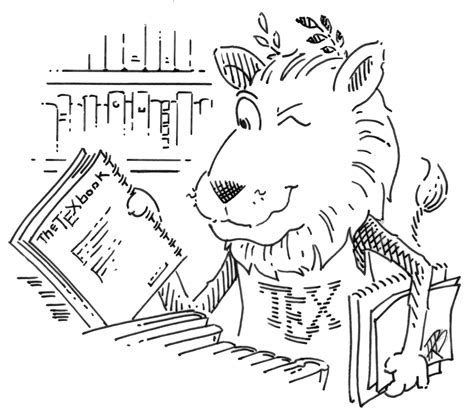
\includegraphics[height=2cm]{lion}
	
\includegraphics[height=2cm]{liang}
	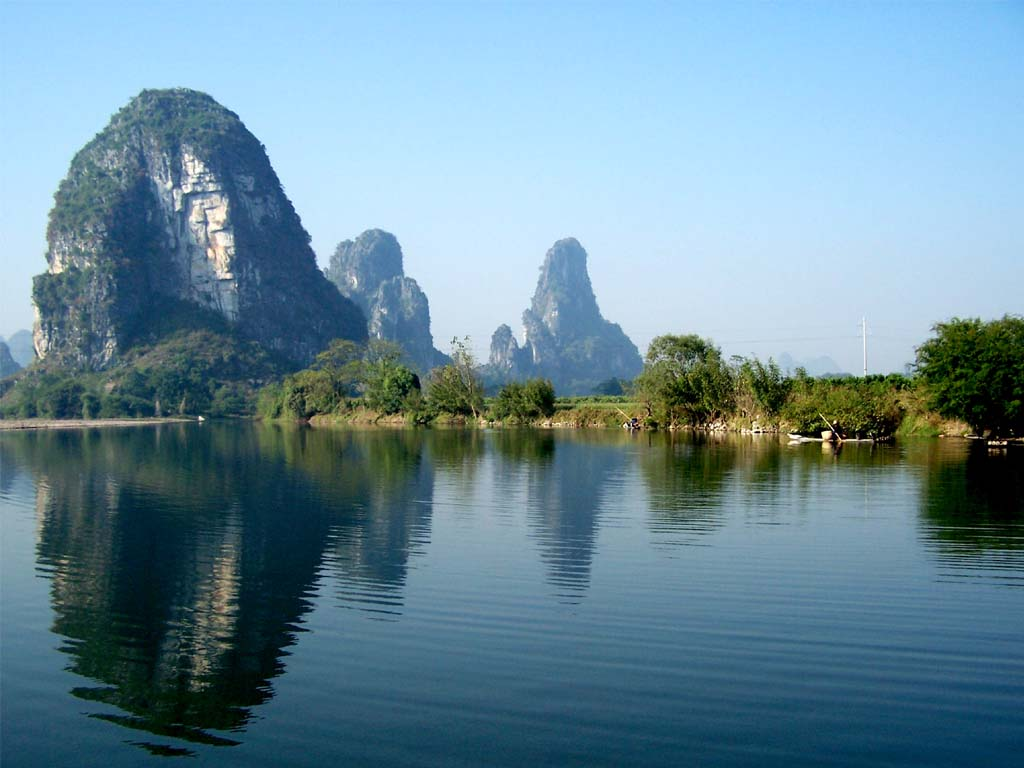
\includegraphics[height=2cm]{guilin}
	
	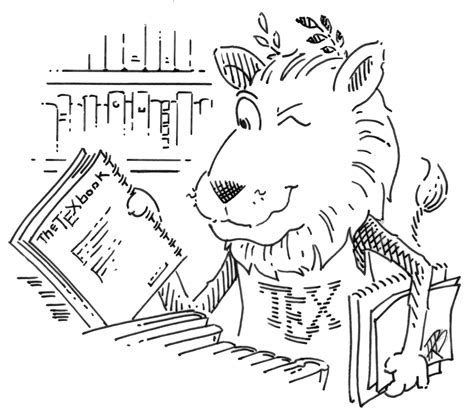
\includegraphics[width=2cm]{lion}
    
\includegraphics[width=2cm]{liang}
    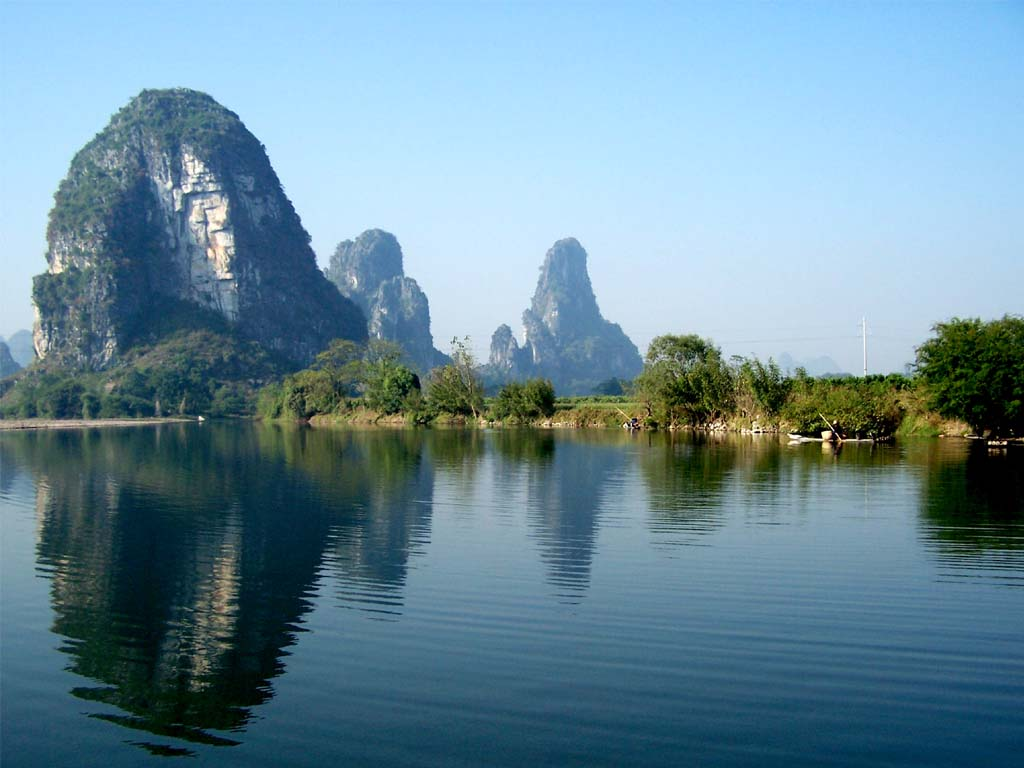
\includegraphics[width=2cm]{guilin}
    
	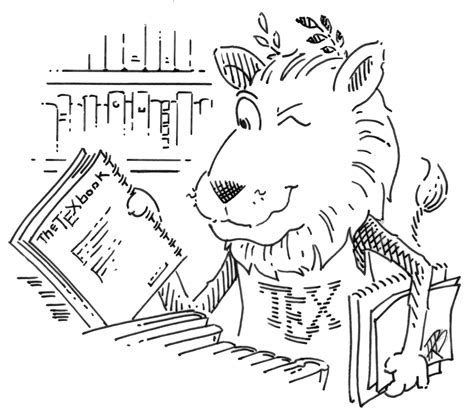
\includegraphics[height=0.1\textheight]{lion}
    
\includegraphics[height=0.1\textheight]{liang}
    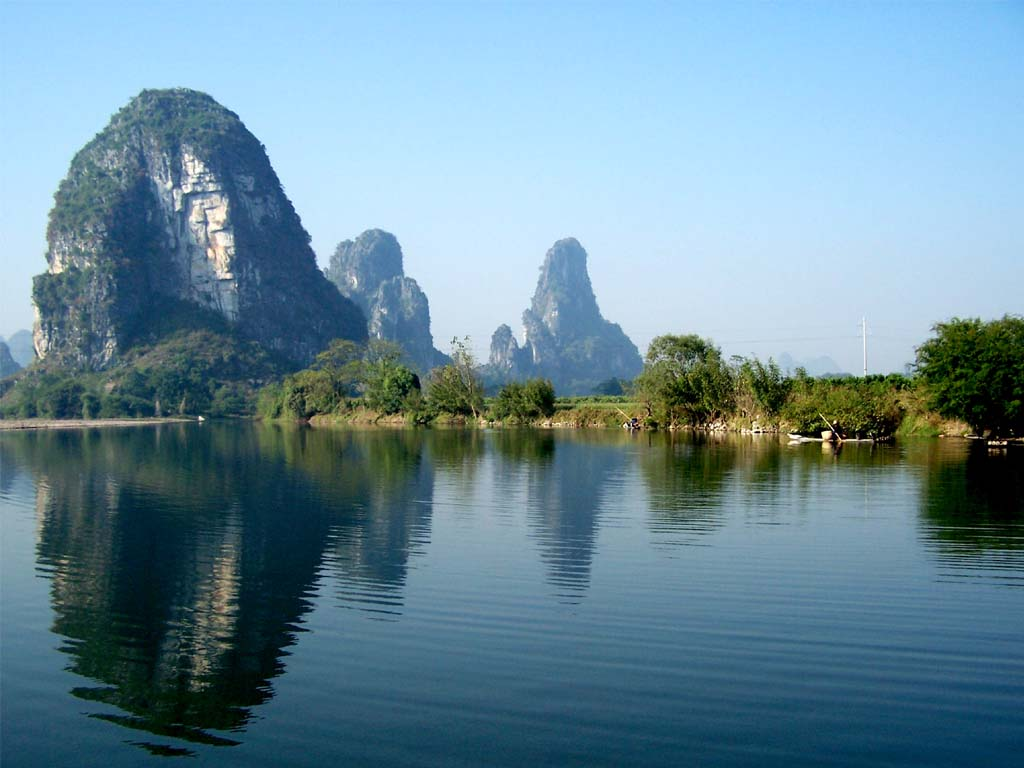
\includegraphics[height=0.1\textheight]{guilin}
    
    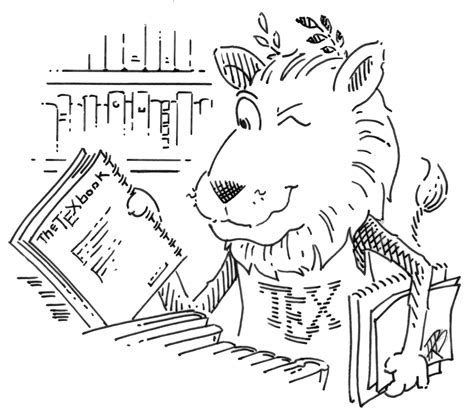
\includegraphics[width=0.2\textwidth]{lion}
    
\includegraphics[width=0.2\textwidth]{liang}
    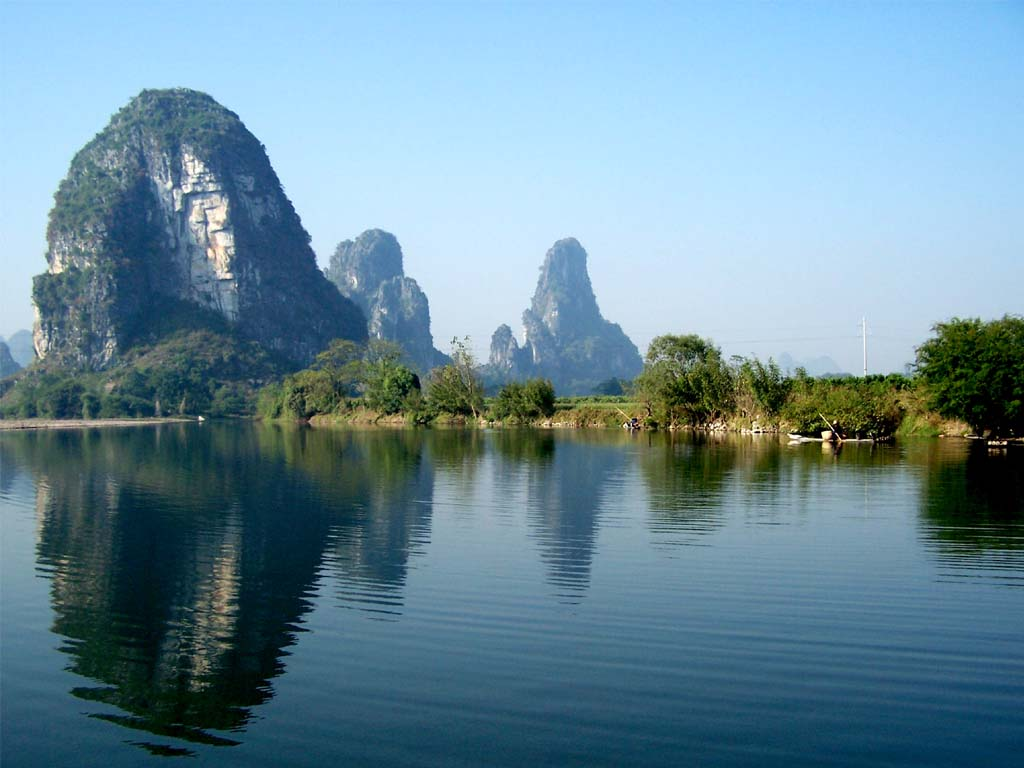
\includegraphics[width=0.2\textwidth]{guilin}  
    
    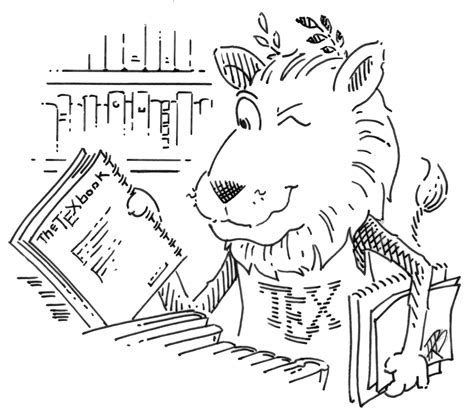
\includegraphics[angle=-45,width=0.2\textwidth]{lion}
    
\includegraphics[width=0.2\textwidth]{liang}
    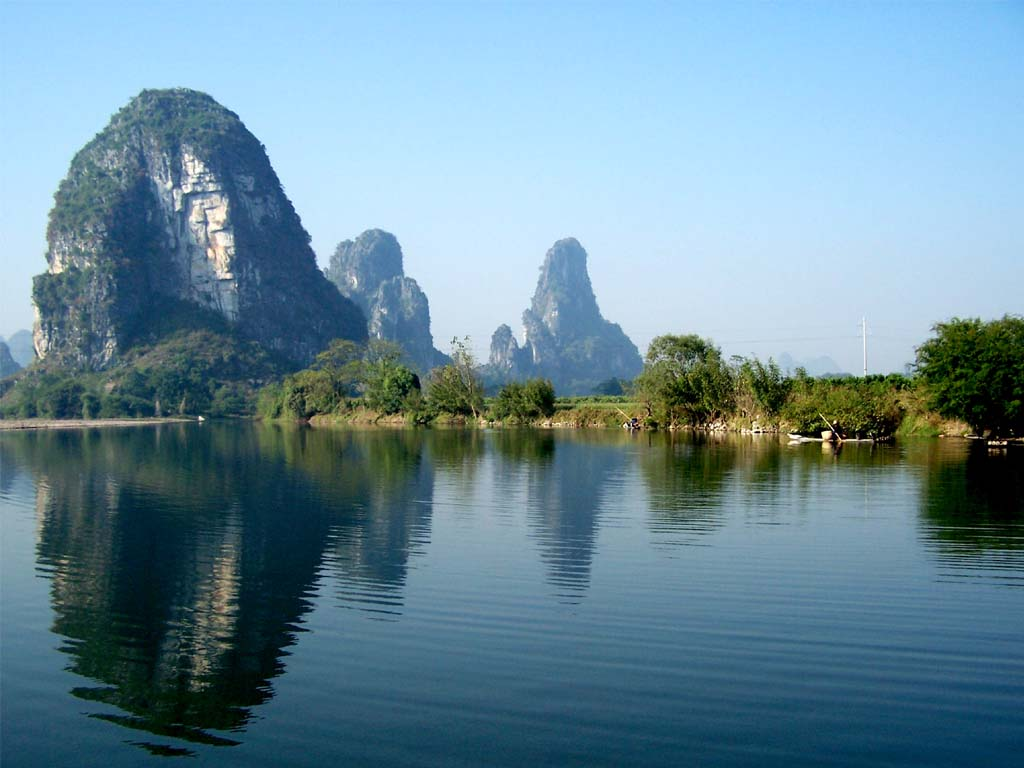
\includegraphics[angle=45,width=0.2\textwidth]{guilin}	
% 帮助文档见 graphicx	
\end{document}